%%% Работа с русским языком
\usepackage{cmap}					% поиск в PDF
\usepackage[T2A]{fontenc}			% кодировка
\usepackage[utf8]{inputenc}			% кодировка исходного текста
\usepackage[english,russian]{babel}	% локализация и переносы
\usepackage{indentfirst}
\frenchspacing

\usepackage{subfigure}

%%% Дополнительная работа с математикой
\usepackage{amsmath,amsfonts,amssymb,amsthm,mathtools} % AMS
\usepackage{icomma} % "Умная" запятая: $0,2$ --- число, $0, 2$ --- перечисление

%%% Работа с картинками
\usepackage{graphicx}  % Для вставки рисунков
\usepackage{wrapfig} % Обтекание рисунков текстом
\usepackage{subfigure}

%%% Работа с таблицами
\usepackage{array,tabularx,tabulary,booktabs} % Дополнительная работа с таблицами
\usepackage{longtable}  % Длинные таблицы
\usepackage{multirow} % Слияние строк в таблице

%%% Программирование
\usepackage{etoolbox} % логические операторы


\usepackage{setspace} % Интерлиньяж
%\onehalfspacing % Интерлиньяж 1.5
%\doublespacing % Интерлиньяж 2
%\singlespacing % Интерлиньяж 1

\usepackage{lastpage} % Узнать, сколько всего страниц в документе.

\usepackage{soul} % Модификаторы начертания

\usepackage{tikz} % Работа с графикой
\usepackage{pgfplots}
\usepackage{pgfplotstable}

\renewcommand{\phi}{\varphi}
\renewcommand{\epsilon}{\varepsilon}
\usepackage[justification=centering, font=footnotesize]{caption}
\setbeamertemplate{caption}[numbered]

\setlength{\parskip}{0.1cm}

\author{Сёмкин Кирилл \and Вадим Стрижов \\ \medskip {\footnotesize Московский Физико-Технический Институт}}
\date{2023}
\title{Тензорный метод SSA в задаче декомпозиции многомерных временных рядов}

\begin{document}
	
	\begin{frame}[c]
		\titlepage
	\end{frame}

	\begin{frame}{Цель исследования}
		
		{
		\begin{alertblock}{Проблема}
			Классические методы декомпозиции временных рядов не позволяют учесть взаимосвязь и общую природу порождения набора временных рядов.
		\end{alertblock}
		}
		
		\begin{block}{Цель}
			Предложить метод, позволяющий выделить общую для набора сигналов структуру, и на её основании произвести разложение на аддитивные компоненты.
		\end{block}
		
		\begin{exampleblock}{Решение}
			Использовать гипотезу порождения рядов общей динамической системой и идею метода SSA. Состыковать траекторные матрицы в тензор, применить каноническое тензорное разложение, на её основе получить декомпозицию типа SVD для каждой матрицы, далее разложить каждый ряд на компоненты.
		\end{exampleblock}
		
	\end{frame}
	
	\begin{frame}{Литература}
		
		\begin{thebibliography}{1}
			
			\bibitem{rabanser2017introduction}
			Stephan Rabanser and Oleksandr Shchur and Stephan Günnemann
			\textit{Introduction to Tensor Decompositions and their Applications in Machine Learning}.
			arXiv, 2017.
			
			\bibitem{ecfb9dc578be43ae9ee8fc88b8ff9151}
			D. Stepanov and N. Golyandin
			\textit{SSA-based approaches to analysis and forecast of multidimensional time series}.
			2005.
			
			\bibitem{6661921}
			Kouchaki, Samaneh and Sanei, Saeid
			\textit{Tensor based singular spectrum analysis for nonstationary source separation}.
			MLSP, 2013.
			
			\bibitem{10122507}
			Fu, Hang and Sun, Genyun and Zhang, Aizhu and Shao
			\textit{Tensor Singular Spectrum Analysis for 3-D Feature Extraction in Hyperspectral Images}.
			IEEE Transactions on Geoscience and Remote Sensing, 2023.
			
		\end{thebibliography}
		
	\end{frame}
	
	\begin{frame}{Постановка задачи}
		
		Пусть имеем набор временных рядов $ \{x_i(t_j)\}_{i = 1}^{m} $, где сетка по времени $ t_j \in \overrightarrow{1, N} $. Стоит задача разложения временных рядов на аддитивные компоненты: 
		
		\begin{gather*}
			x_1(t) = f_1(t) + f_2(t) + \ldots + f_{n_1}(t) \\
			x_2(t) = g_1(t) + g_2(t) + \ldots + g_{n_2}(t) \\
			...
		\end{gather*}
		
			\begin{alertblock}{Проблема}
				
				Способов разложения бесконечно много, нужно конкретизировать требования на компоненты $ f_i(t), g_i(t) $ и т.д.
				
			\end{alertblock}
		
	\end{frame}
	
	\begin{frame}{Метод SSA}
		
		\only<1>{
			Имеем один временной ряд. Предполагаем его порождение некоторой (скрытой) динамической системой, используем теорему Такенса для её восстановления.
			
			Выбираем длину окна $ L $, строим \textit{вектора задержек}  $ \mathbf{x}_k = ( x(t_k) \  x(t_{k+1}) \  \ldots \  x(t_{k + L - 1}) ) $, собираем их по столбцам в ганкелеву матрицу $ T $ (\textit{траекторная матрица}).
		}
		
		\only<2>{
			Далее к матрице применяется SVD-разложение $ T = \sum\limits^{r} \sigma_i \mathbf{u}_i \mathbf{v}_i $
			
			Предполагается существование разбиение факторов на 2 (или более) группы так, что $ T = X_1 + X_2 $, причём $ X_1, X_2 $ - также траекторные матрицы некоторых сигналов $ f_1(t), f_2(t) \Rightarrow x(t) = f_1(t) + f_2(t) $
		}
		 
		\only<1-2>{
		\begin{figure}
			\centering
			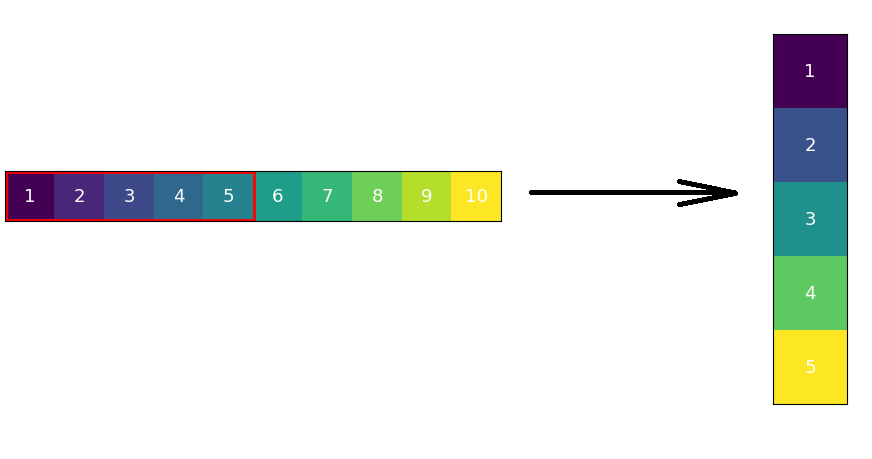
\includegraphics[width=0.45\textwidth, keepaspectratio]{../../figs/first_round}
			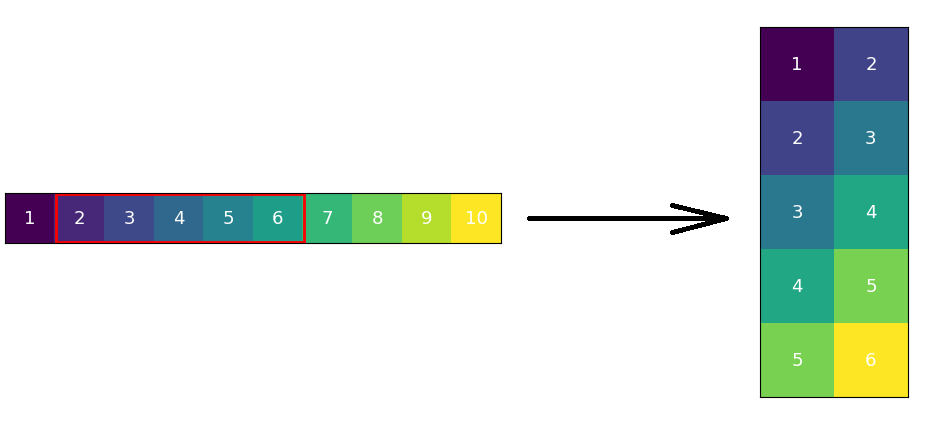
\includegraphics[width=0.45\textwidth, keepaspectratio]{../../figs/second_round.png}
			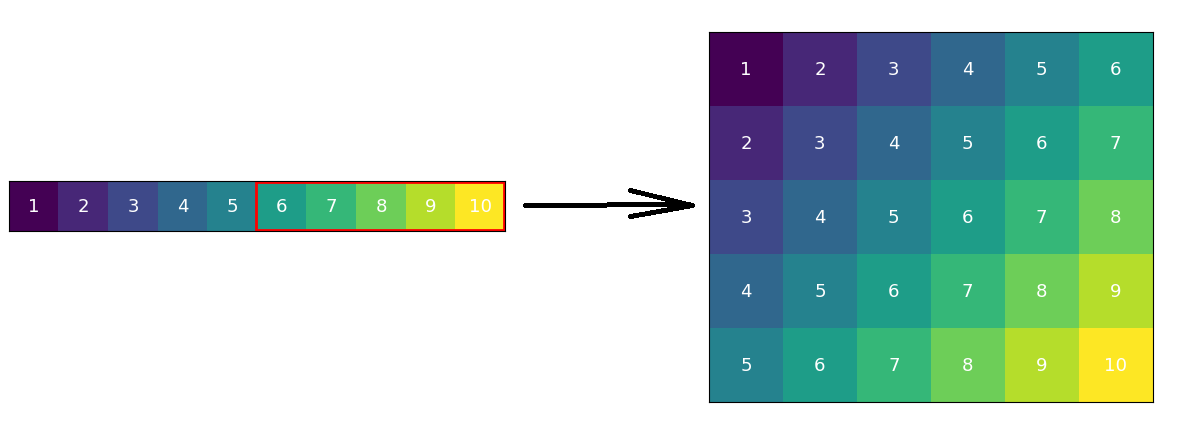
\includegraphics[width=0.45\textwidth, keepaspectratio]{../../figs/last_round.png}
			\caption{Построение траекторной матрицы}\label{pic:hankel_build}
		\end{figure}
	}
		
	\end{frame}
	
	\begin{frame}{Метод mSSA}
		
		Имеем набор временных рядов. Строим траекторные матрицы для каждого ряда $ T_1, T_2, \ldots , T_m  $, конкатенируем все матрицы в одну $ T = [T_1 \  T_2 \ldots T_m] $, которую далее раскладываем с помощью SVD
		
		
		\begin{figure}
			\centering
			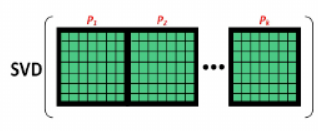
\includegraphics[width=0.45\textwidth, keepaspectratio]{../../figs/mSSA_demonst.png}
			\caption{Метод mSSA}\label{pic:mSSA_dem}
		\end{figure}
		
		\begin{equation*}
			T = \sum\limits_i^{r} \sigma_i \mathbf{u}_i \mathbf{v}_i \Leftrightarrow \begin{cases}
				T_1 = \sum\limits_i^{r} \sigma_i \mathbf{u}_i \mathbf{v}_i^1 \\
				T_2 = \sum\limits_i^{r} \sigma_i \mathbf{u}_i \mathbf{v}_i^2 \\
				\ldots \\
				T_m = \sum\limits_i^{r} \sigma_i \mathbf{u}_i \mathbf{v}_i^m
			\end{cases}
		\end{equation*}
		
	\end{frame}
	
	\begin{frame}{Метод tSSA}
		
		Теперь состыкуем матрицы по третьему измерению, получим траекторный тензор $ \mathbf{T} $. Применим CPD-разложение:
		
		\begin{figure}[h]
			\centering
			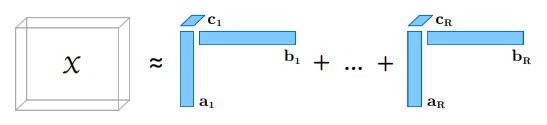
\includegraphics[width=0.48\textwidth, keepaspectratio]{../../figs/cpu_decomp}
			\caption{Иллюстрация CPD разложения}\label{pic:cpu_dec}
		\end{figure}
		
		С математической точки зрения это выглядит так:
		
		\begin{equation*}
			\mathbf{T} = \sum\limits_i^{r} \mathbf{a}_i \otimes \mathbf{b}_i \otimes \mathbf{c}_i \Leftrightarrow \begin{cases}
				T_1 = \sum\limits_i^{r} \mathbf{c}_i[1] \cdot \mathbf{a}_i  \mathbf{b}_i  \\
				T_2 = \sum\limits_i^{r} \mathbf{c}_i[2] \cdot \mathbf{a}_i  \mathbf{b}_i \\
				\ldots \\
				T_m = \sum\limits_i^{r} \mathbf{c}_i[m] \cdot \mathbf{a}_i  \mathbf{b}_i 
			\end{cases}
		\end{equation*}
		
	\end{frame}
	
	\begin{frame}{Вычислительный эксперимент}
		
		\textbf{Цель вычислительного эксперимента}: сравнить работу методов mSSA и tSSA на синтетических (набор синусов с разными фазами) и на реальных временных рядах (акселерометрия). 
		
		\textit{Метрики качества}:
		
		\begin{itemize}
			
			\item интерпретируемость компонент разложения
			
			\item расхождение исходных рядов от суммы полученных декомпозиций
			
		\end{itemize}
		
	\end{frame}
	
	\begin{frame}{Синтетические данные}
		
		\only<1>{
			
			Сгенерирован набор $ x_i(t) = \sin(w_i \cdot t) + \epsilon_i $, где $ w_i \in \{1, 2, 3\} $ - частоты, $ \epsilon_i $ - небольшой гауссовский шум.
			
		}
		
		\only<2>{
			
			\begin{figure}
				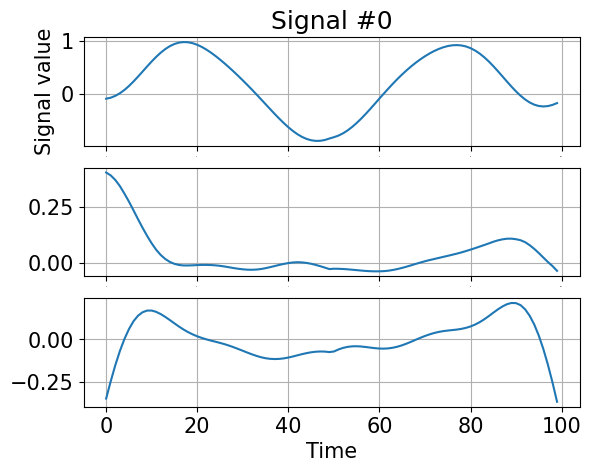
\includegraphics[width=0.4\textwidth, keepaspectratio]{img/mssa_sines_comps.png}
				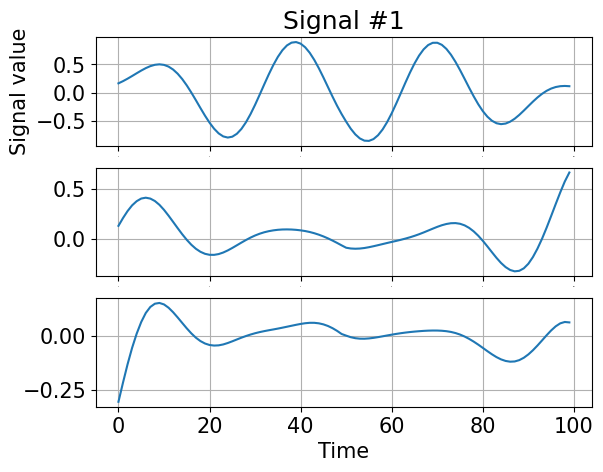
\includegraphics[width=0.4\textwidth, keepaspectratio]{img/mssa_sines_comp1.png}
				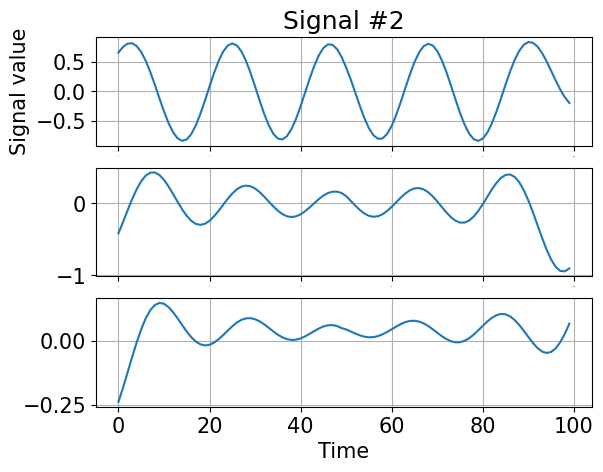
\includegraphics[width=0.4\textwidth, keepaspectratio]{img/mssa_sines_comp2.png}
				\caption{Метод mSSA. Разложение рядов на компоненты}
			\end{figure}
			
		}
		
		\only<3>{
			
			\begin{figure}
				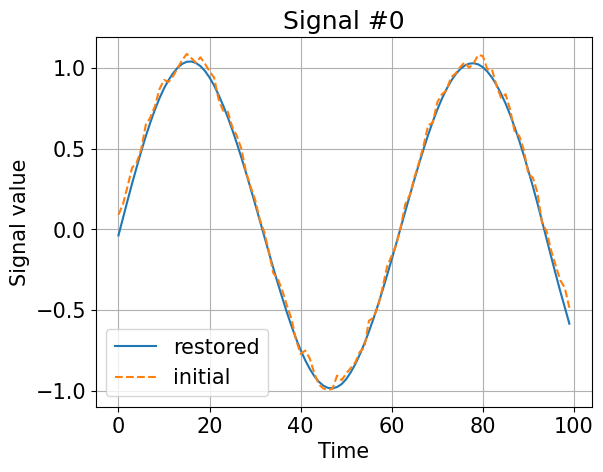
\includegraphics[width=0.4\textwidth, keepaspectratio]{img/mssa_sines_compar.png}
				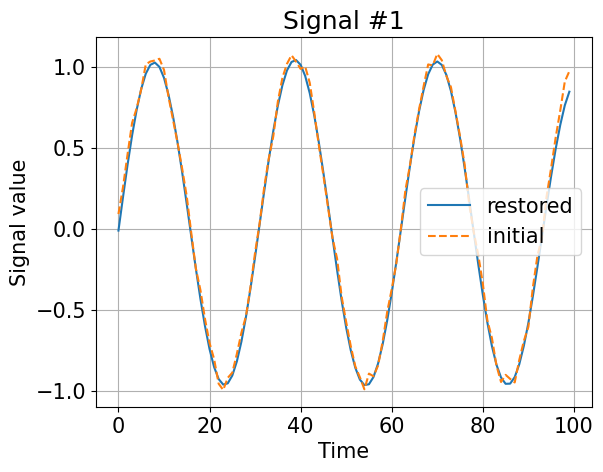
\includegraphics[width=0.4\textwidth, keepaspectratio]{img/mssa_sines_compar1.png}
				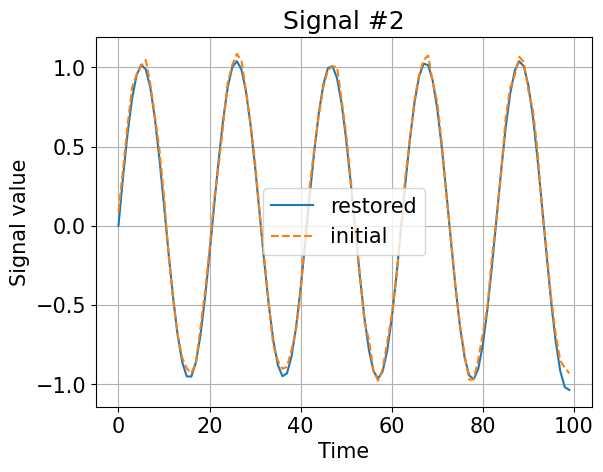
\includegraphics[width=0.4\textwidth, keepaspectratio]{img/mssa_sines_compar2.png}
				\caption{Метод mSSA. Сопоставление истинного ряда и его аппроксимации}
			\end{figure}
			
		}
		
	\end{frame}
	
	\begin{frame}{Синтетические данные}
		
		\only<1>{
			
			\begin{figure}
				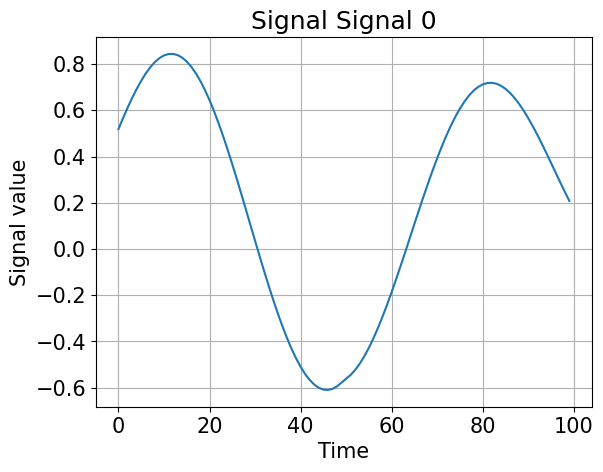
\includegraphics[width=0.4\textwidth, keepaspectratio]{img/tssa_sines_comp1.png}
				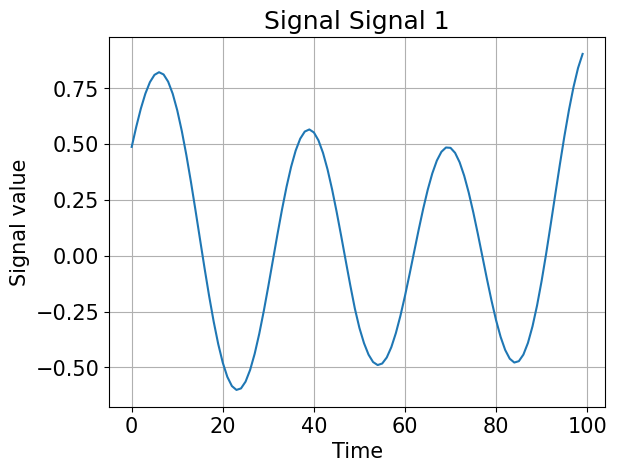
\includegraphics[width=0.4\textwidth, keepaspectratio]{img/tssa_sines_comp2.png}
				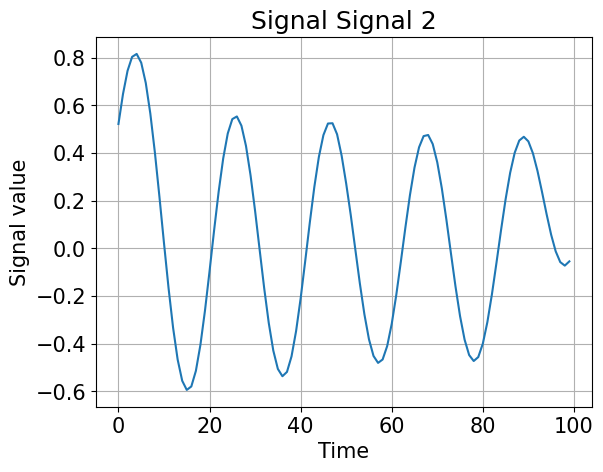
\includegraphics[width=0.4\textwidth, keepaspectratio]{img/tssa_sines_comp3.png}
				\caption{Метод tSSA. Разложение рядов на компоненты}
			\end{figure}
			
		}
		
		\only<2>{
			
			\begin{figure}
				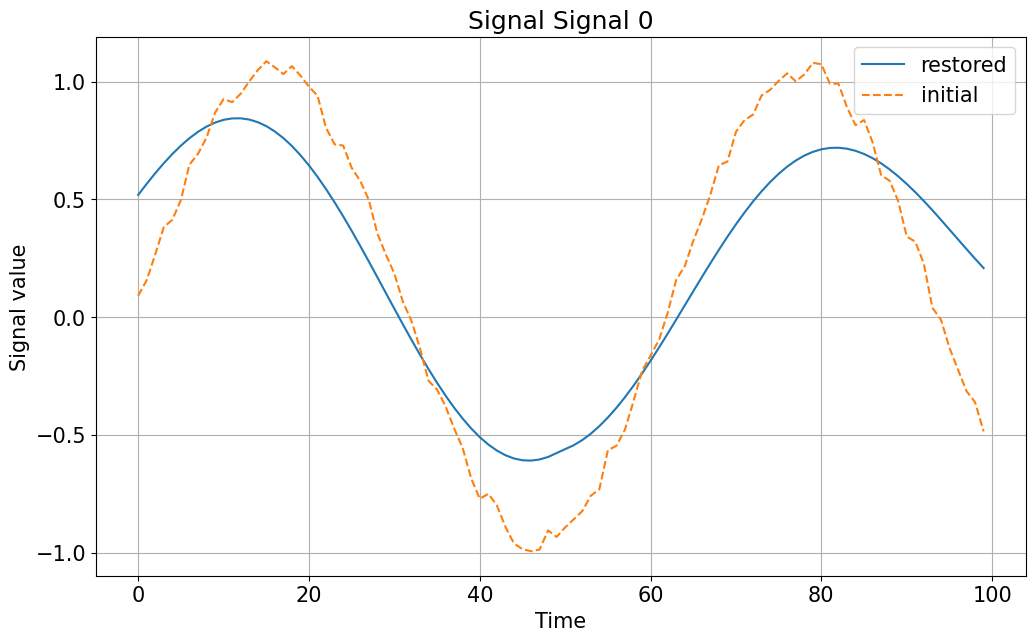
\includegraphics[width=0.4\textwidth, keepaspectratio]{img/tssa_sines_compar1.png}
				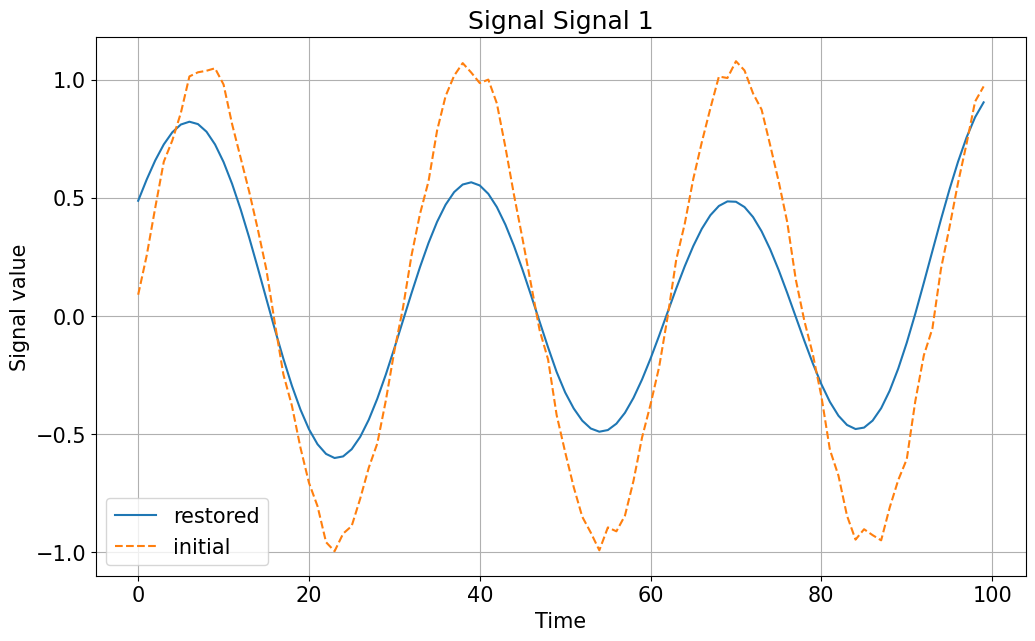
\includegraphics[width=0.4\textwidth, keepaspectratio]{img/tssa_sines_compar2.png}
				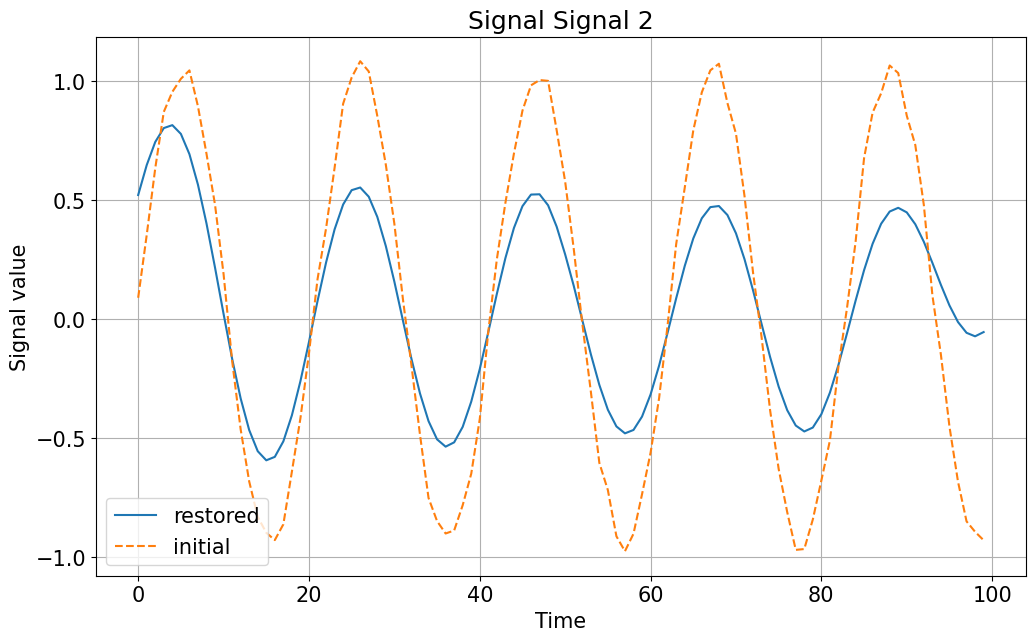
\includegraphics[width=0.4\textwidth, keepaspectratio]{img/tssa_sines_compar3.png}
				\caption{Метод tSSA. Сопоставление истинного ряда и его аппроксимации}
			\end{figure}
			
		}
		
	\end{frame}
	
	\begin{frame}{Акселерометрия}
		
		\only<1>{
			
			Имеем три временных ряда  --- компоненты вектора ускорения идущего человека.
			
			\begin{figure}
				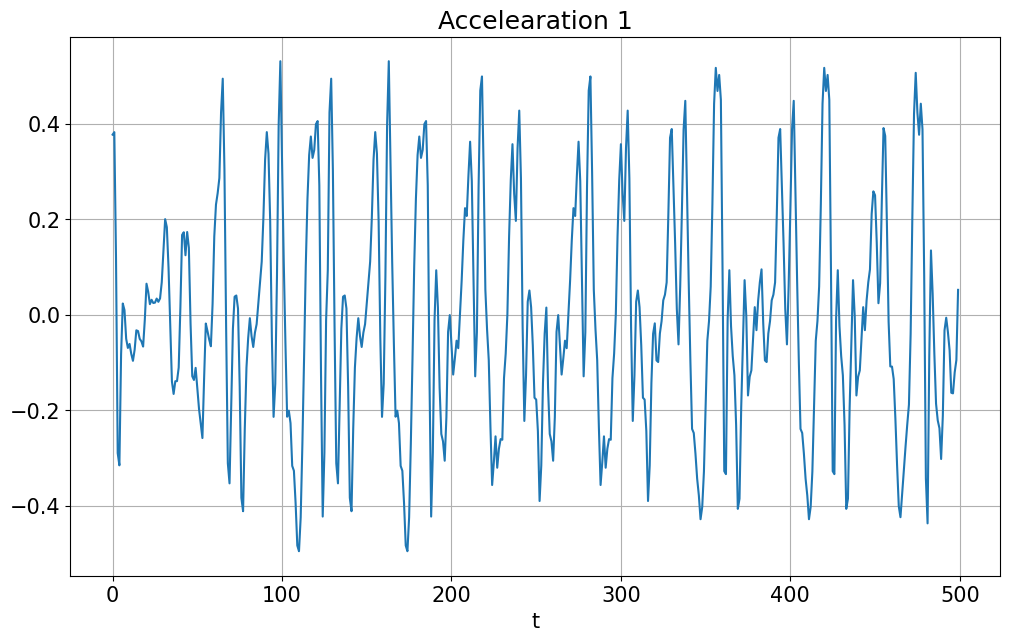
\includegraphics[width=0.45\textwidth, keepaspectratio]{img/acceler_1.png}
				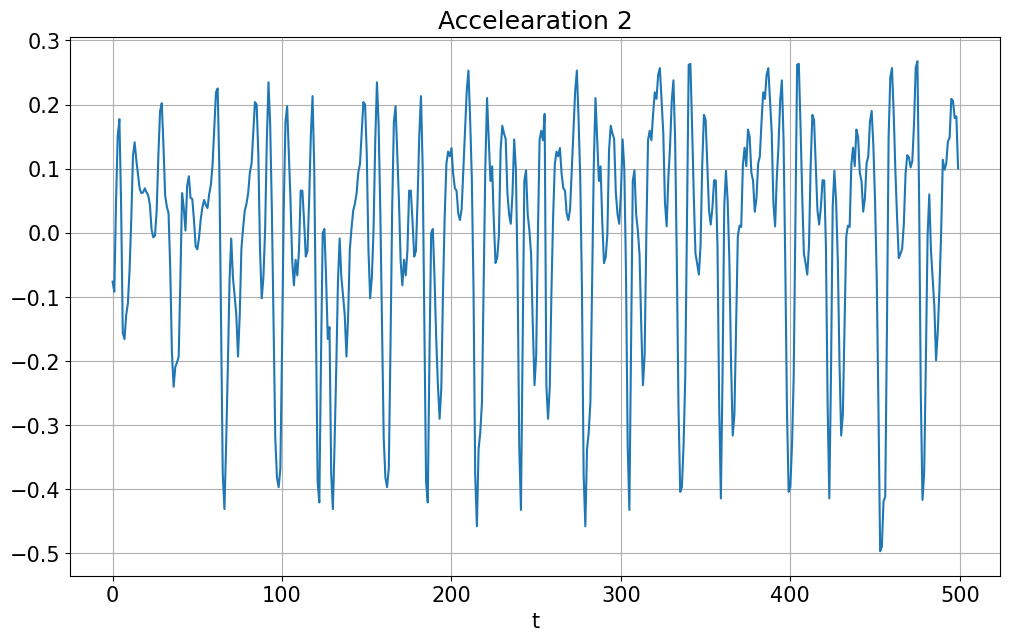
\includegraphics[width=0.45\textwidth, keepaspectratio]{img/acceler_2.png}
				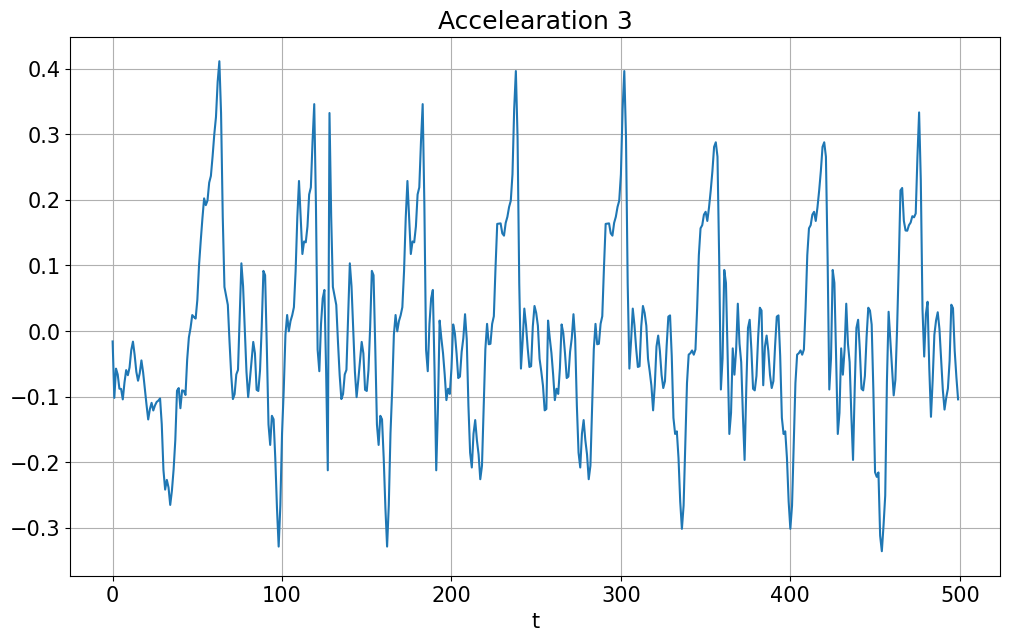
\includegraphics[width=0.45\textwidth, keepaspectratio]{img/acceler_3.png}
			\end{figure}
			
		}
		
		\only<2>{
			
			\begin{figure}
				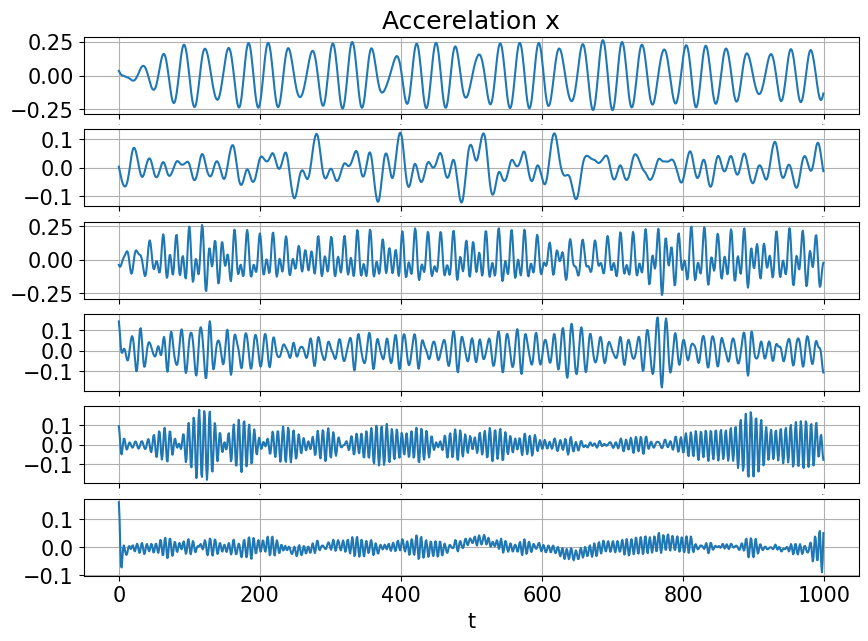
\includegraphics[width=0.4\textwidth, keepaspectratio]{img/mssa_acceler_comp1.png}
				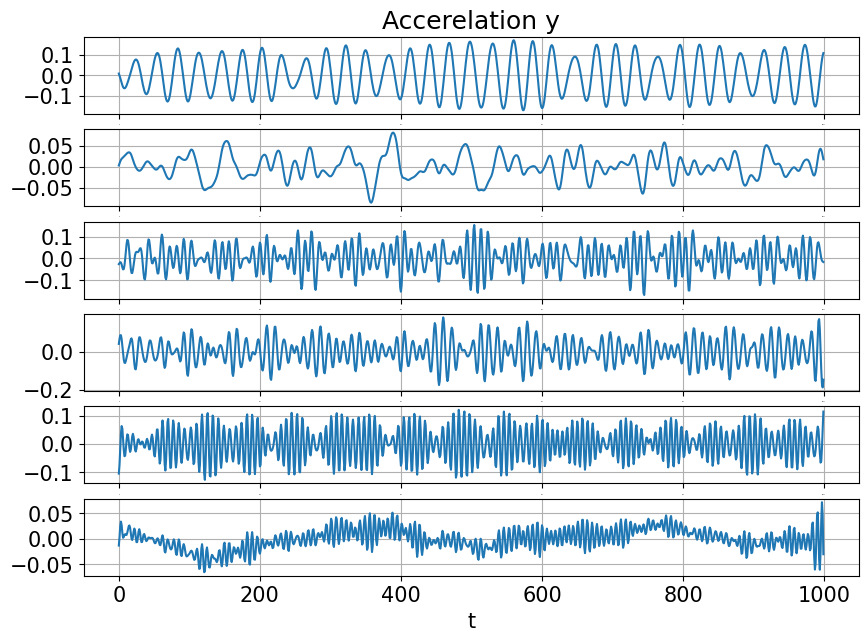
\includegraphics[width=0.4\textwidth, keepaspectratio]{img/mssa_acceler_comp2.png}
				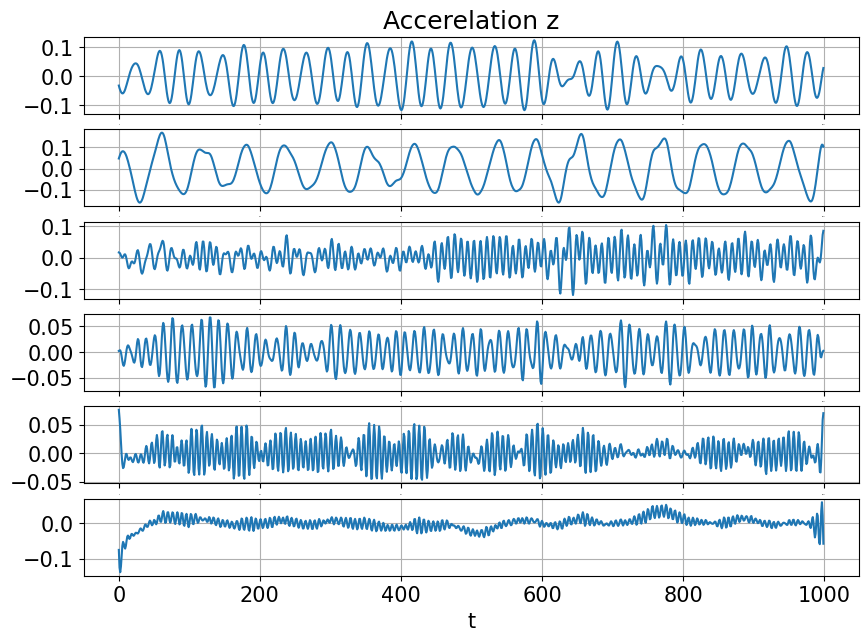
\includegraphics[width=0.4\textwidth, keepaspectratio]{img/mssa_acceler_comp3.png}
				\caption{Метод mSSA. Разложение рядов на компоненты}
			\end{figure}
			
		}
		
		\only<3>{
			
			\begin{figure}
				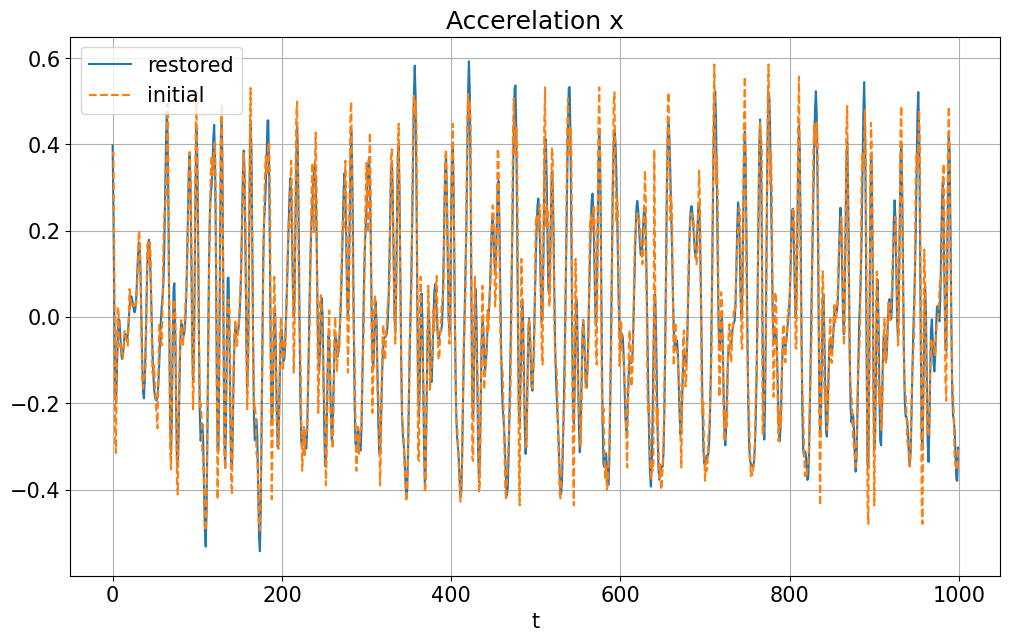
\includegraphics[width=0.4\textwidth, keepaspectratio]{img/mssa_acceler_compar1.png}
				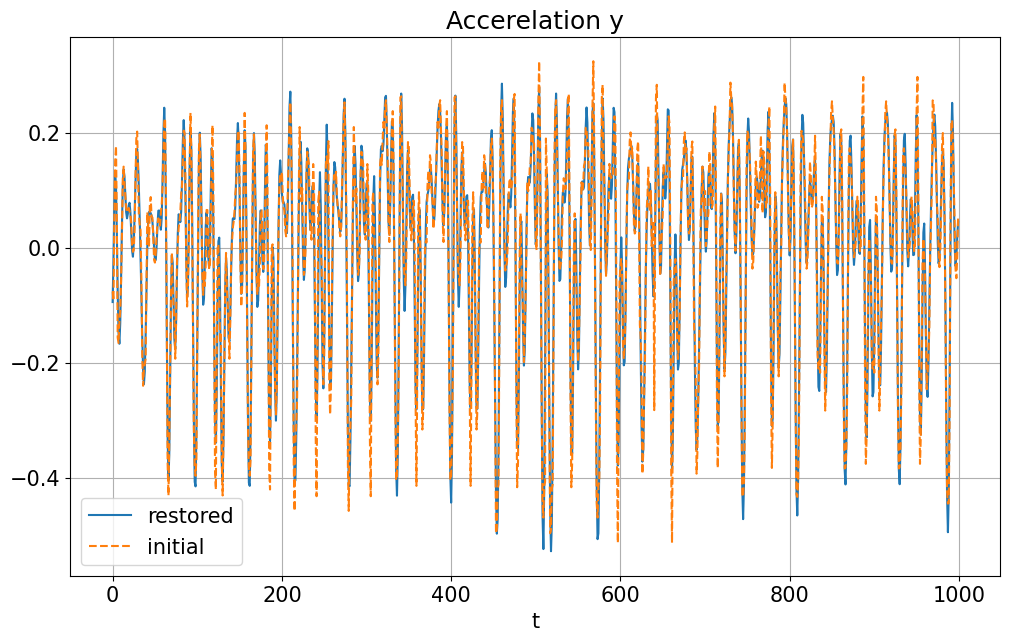
\includegraphics[width=0.4\textwidth, keepaspectratio]{img/mssa_acceler_compar2.png}
				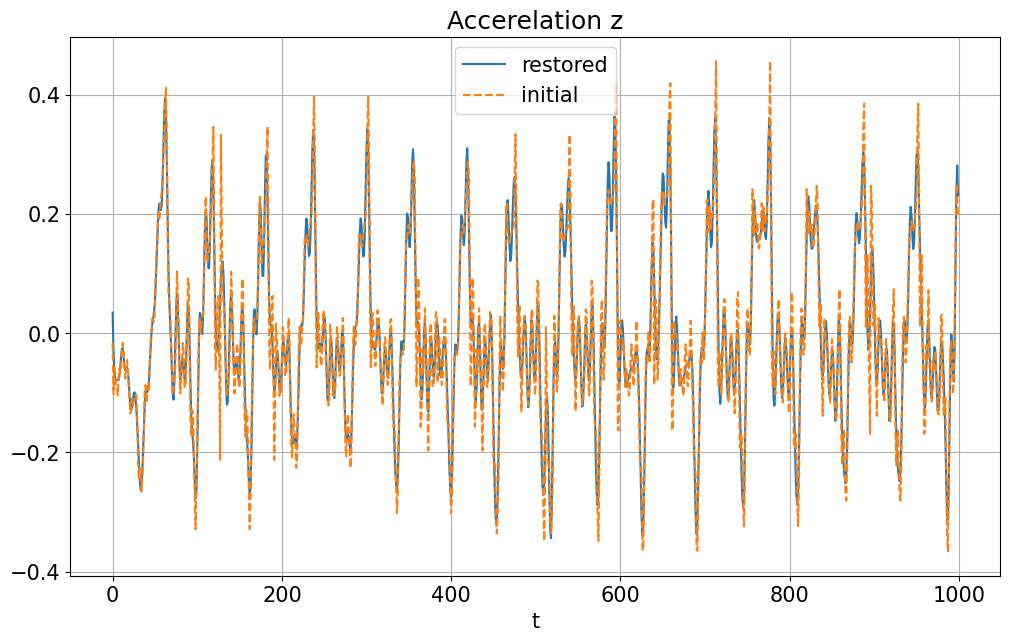
\includegraphics[width=0.4\textwidth, keepaspectratio]{img/mssa_acceler_compar3.png}
				\caption{Метод mSSA. Сопоставление истинного ряда и его аппроксимации}
			\end{figure}
			
		}
		
	\end{frame}
	
	\begin{frame}{Акселерометрия}
		
		\only<1>{
			
			\begin{figure}
				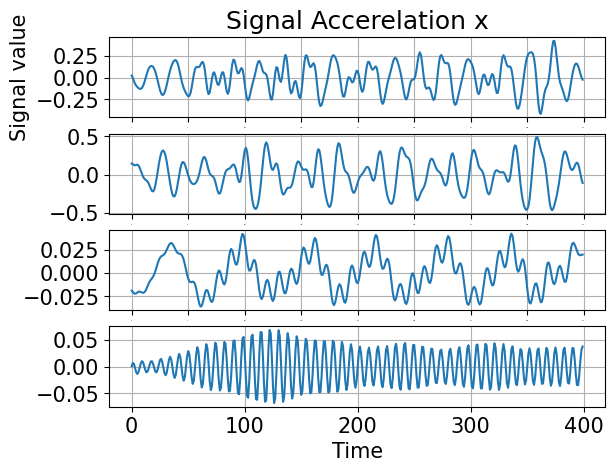
\includegraphics[width=0.4\textwidth, keepaspectratio]{img/tssa_acceler_comp1.png}
				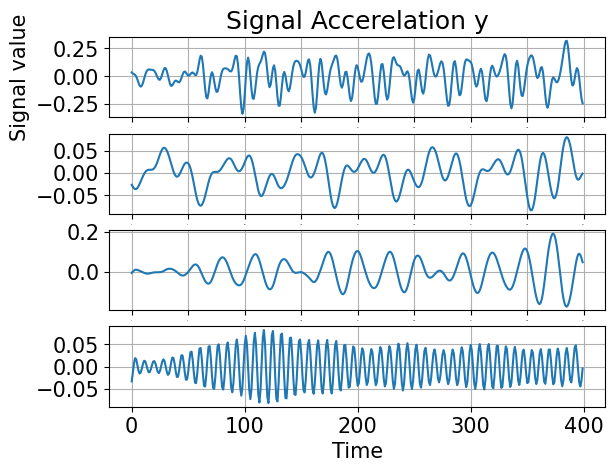
\includegraphics[width=0.4\textwidth, keepaspectratio]{img/tssa_acceler_comp2.png}
				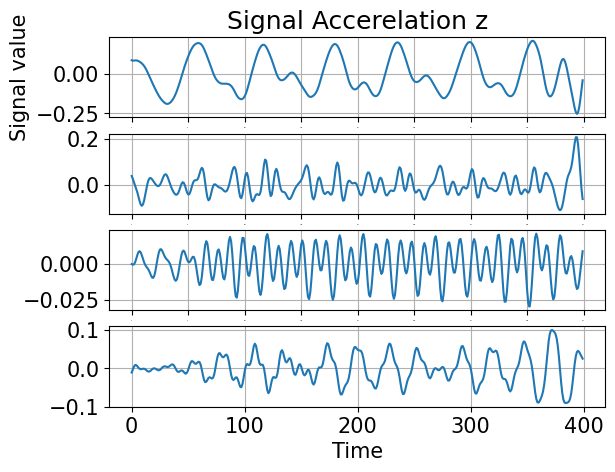
\includegraphics[width=0.4\textwidth, keepaspectratio]{img/tssa_acceler_comp3.png}
				\caption{Метод tSSA. Разложение рядов на компоненты}
			\end{figure}
			
		}
		
		\only<2>{
			
			\begin{figure}
				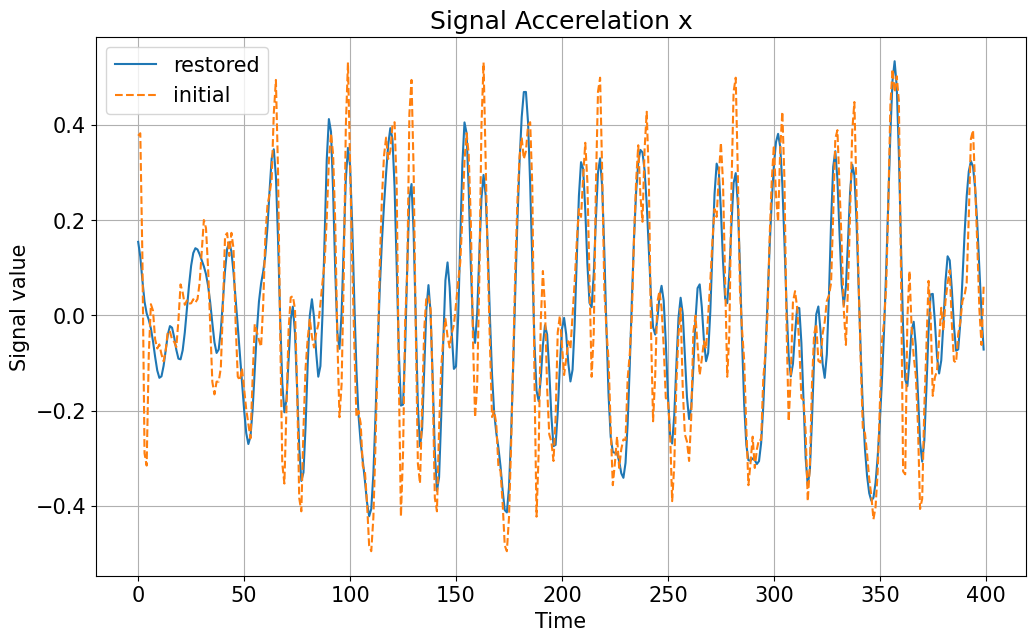
\includegraphics[width=0.4\textwidth, keepaspectratio]{img/tssa_acceler_compar1.png}
				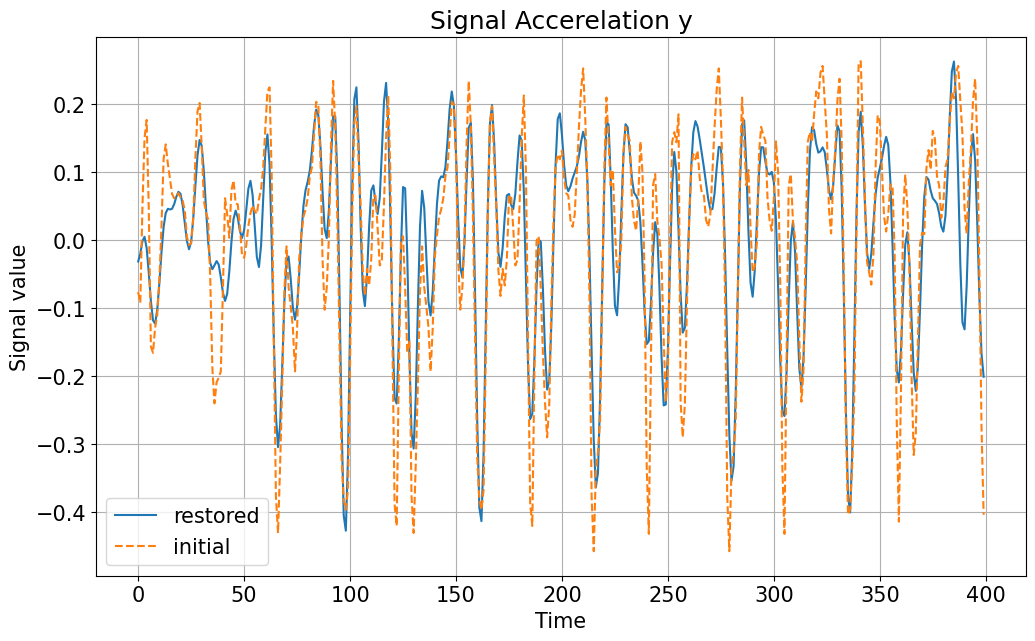
\includegraphics[width=0.4\textwidth, keepaspectratio]{img/tssa_acceler_compar2.png}
				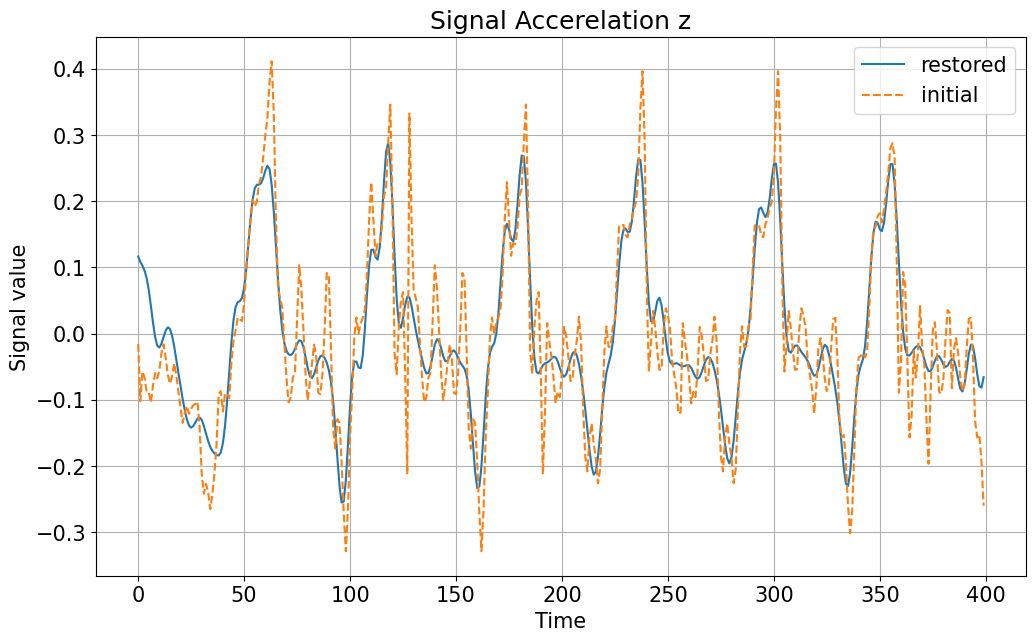
\includegraphics[width=0.4\textwidth, keepaspectratio]{img/tssa_acceler_compar3.png}
				\caption{Метод tSSA. Сопоставление истинного ряда и его аппроксимации}
			\end{figure}
			
		}
		
	\end{frame}
	
	\begin{frame}{Анализ ошибки}
		
		\begin{itemize}
			\item оба метода смогли вычленить сложные составляющие рядов, в том числе модулированные сигналы
			
			\item точность аппроксимации tSSA пока получается ниже, чем у mSSA
			
			\item тем не менее tSSA намного гибче в плане выбора компонент для каждого сигнала
		\end{itemize}
		
	\end{frame}
	
	\begin{frame}{Дальнейшая работа}
		
		Далее планируется внести поправки в алгоритм tSSA, продолжить его математический анализ, усложнить рассматриваемую модель, провести больше экспериментов.
		
	\end{frame}

	
	
\end{document}